\begin{figure*}[tp]
  \centering
  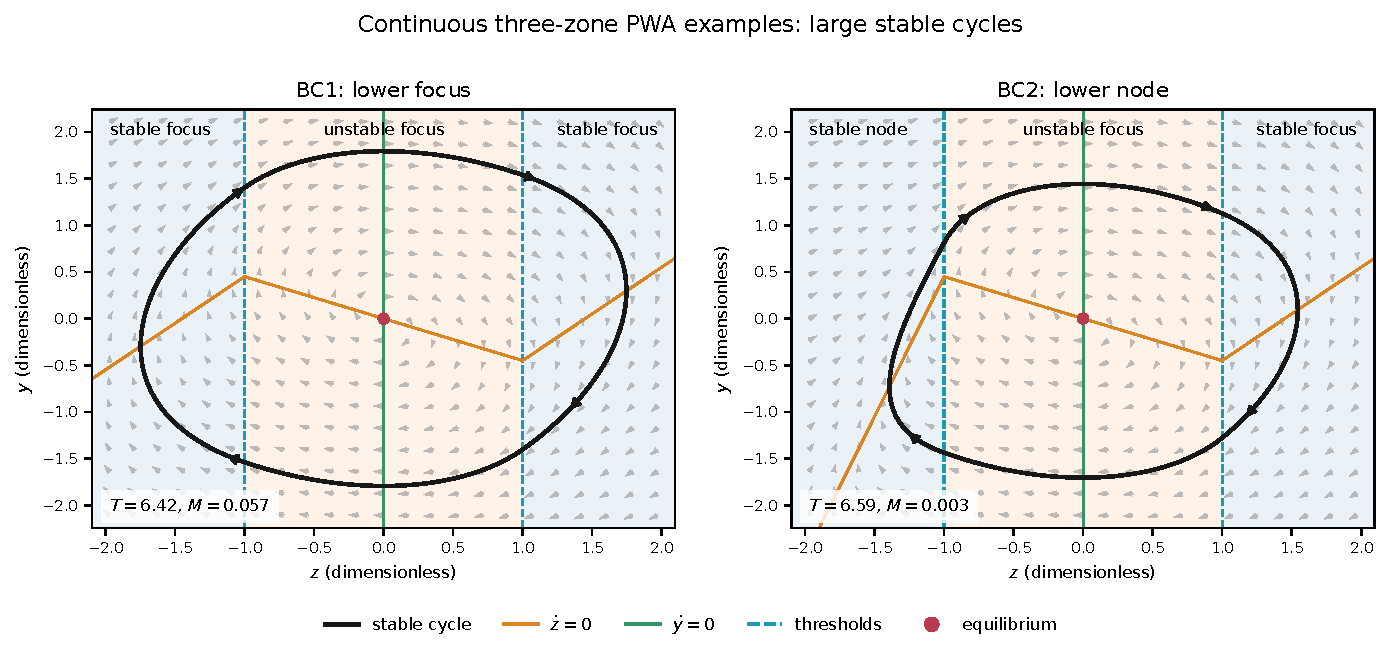
\includegraphics[width=\textwidth,height=.73\textheight,keepaspectratio]{figures/figure4_large_cycles.pdf}
  \caption{Numerically computed phase portraits for two dimensionless continuous three-zone PWA examples. The equations are $\dot z=y-F(z)$, $\dot y=-z$, with thresholds $z=\pm 1$ and continuous piecewise-linear $F(0)=0$. The slopes of $F$ from left to right are $(1,-0.45,1)$ for BC1 and $(3,-0.45,1)$ for BC2. The black curves are attracting periodic orbits crossing both thresholds; grey arrows indicate the normalized vector field, and orange and green lines show the nullclines. $T$ is the period and $M$ the nontrivial Floquet multiplier from the divergence integral. Region labels describe the corresponding affine dynamics; only the point at the origin is an actual equilibrium. These constructed examples are not fitted Li--Rinzel models.}
  \label{fig:large-cycles}
\end{figure*}
